

% ==============================================================================
% START: Introduction
% ==============================================================================
\section{Introduction}

\subsection{Ethereum Blockchain technology}
Blockchain technology was introduced to the general public in 2009 with the cryptocurrency Bitcoin \cite{swan2015blockchain} as a way of transfer/represent value in a decentralized auto-regulated network with the same name (Bitcoin network) as a consequence no single human nor government could control or regulate the exchange of digital assets. The Bitcoin network could be defined as a distributed database that contains encrypted information of the ownership of its unit value, namely the Bitcoin, a detailed explanation can be found in Satoshi Nakamoto's legendary white paper \cite{nakamoto2008bitcoin}. Let us now introduce a example of a operation on the Bitcoin network that will be generalized for Etherum network.

\begin{itemize}
	\item Let there be two users of the Bitcoin network, this network is composed of nodes, each node has a single exact copy of the database. 
	\item Both subjects have a private and a public cryptographic key, in the community these pair is referred to as a wallet. In reality, it can be viewed as a record on the public database stating that those private keys are associated with $x \in \mathbb{R}^{\geq0}$ and $y \in \mathbb{R}^{\geq0}$  Bitcoin units.
	\item If user A tries to reassign its $x$ Bitcoin to user B, the Bitcoin network must reach a consensus. First, a validation of the claim \emph{User A has $x$ Bitcoins} must be verified by all the nodes in the network, this done just by checking in the local copy of the database if \emph{User A has $x$ Bitcoins} .
	\item After this validation, each node would compete to gain the right to \emph{write} this new transaction to their local database and then broadcast to the other nodes. In the first implementations, this was done by iteratively passing a string representation of the operation to a hashing function until the outcome had the first $N$ characters equal to 0. Nodes that actively seek to claim the right to update the database were commonly refers to as miners, and the reward for winning this competition would be the assignation of newly created Bitcoin to the miner wallet.
	\item The network has some extra coded features, such that the rate of updates of the database cannot exceed a threshold dictated by the number of actives nodes. By adjusting the degree of difficulty, in our example, the $N$ characters beginning with zero, the supply of cryptocurrency gets regulated. 
\end{itemize}

The previous example is just illustrative, there are many more complications regarding any Blockchain, however, we consider that it serves the purpose of introducing terminology in a straight forward manner to a nontechnical reader. For a quite pleasant technical overview of the subject, please refer to \cite{vujivcic2018blockchain}.\\

Vitalik Buterin introduced the Ethereum network in the white paper \cite{buterin2014ethereum} to extend the   Bitcoin network functionality by implementing a \emph{Turing-complete programming  language} as a consequence any node of the network is no longer limited to store a copy of the database but can also create its own \emph{owernship rules, formats of  transactions,  and  state  transition  functions} \cite{vujivcic2018blockchain}. When a node defines its own rules, any other node can choose to enter the \emph{contract} that would self execute according to the logical rules written in it. With this new artifact, users can create self-executing digital contracts whose unit values(the \emph{Ether}) are publicly available for auditing while preserving the privacy of the users.\\

In addition to the intended use of the Ethereum Network from the prior discussion, there are platforms such as \emph{Bitstamp} in Europe, \emph{Coinbase} in the U.S.A, and \emph{Bitso} in Mexico where users can speculate over the value of any cryptocurrency against any \emph{fiat} such as the Euro, Dollar or Mexican Peso. It should be noticed that in these \emph{exchanges} when a client buys a token using his or her fiat money, the blockchain in which that token represent value does not get updated as in our example. Instead, the ownership of the token gets updated inside the private records of the exchange giving the illusion of instant transference times. Only when the user decides to take his or her cryptocurrencies out of the exchange into his own private wallet, for example, the involved Network gets updated.\\

There are two crucial considerations that ultimately motivate an attempt to predict the average price of the following day of the token Ether. First, we believe that \emph{Smart contracts} applications depicts an excellent future for the long term value of the token, so investing in an intraday fashion is a subjectively risk reduced enterprise. Second, by perfecting a predicting technique, a risk reduced fiat market opens for the modeler, since a token can be freely moved between different exchanges that have separate fiat counterparts.


\begin{table}[h!]
\begin{center}
\begin{tabular}{||c c c  c||} 
\hline
Name & Market Capitalization & Price  & Circulating supply\\ [0.5ex] 
\hline\hline
Bitcoin & \$139,157,553,209 & \$7,856.69& 17,711,975 BTC \\ 
\hline
Ether& \$26,234,724,752 & \$247.15 &  106,148,488 ETH  \\ 
\hline
XRP & \$16,517,864,972 & \$0.392038 &  42,133,310,721 XRP  \\
\hline
\end{tabular}
\caption{Principal economics indicator for Cryptocurrency against USD. Taken from \cite{coin}}
\label{table:cripto_markets}
\end{center}
\end{table}




\subsection{Data Sources}

Two sources of data were used throughout the present dissertation. Namely \textbf{Ether Scan} \cite{ether_scan} specifically the price and daily transactions charts and the \textbf{Deepblue Bot} \cite{deepblueai} for social media information regarding the Ethereum Network. 

% Including figures
\begin{figure}[htpb!] % Defines figure environment
	\centering % Centers your figure
	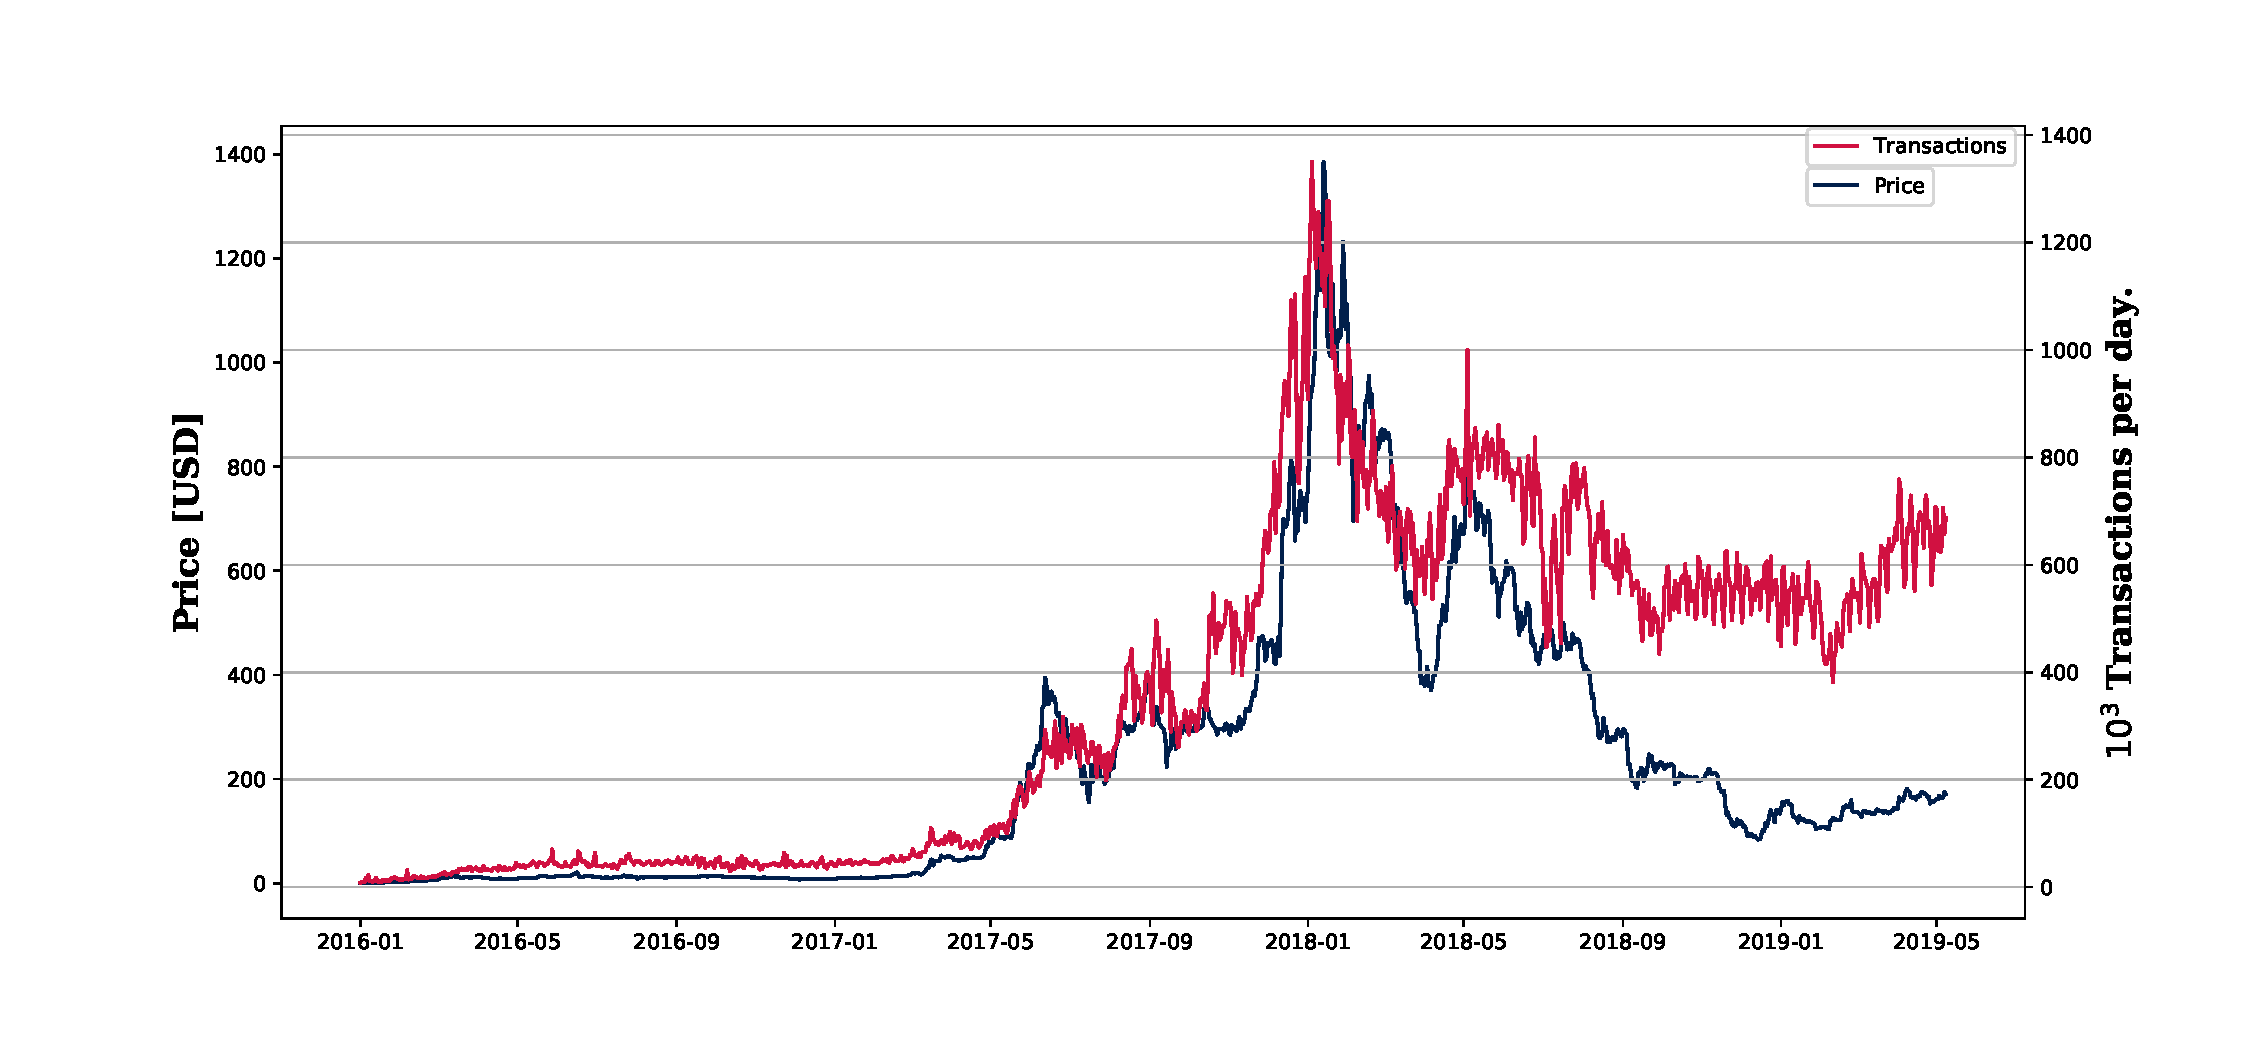
\includegraphics[width=\textwidth]{data/ether_scan_price_trans.pdf} % Includes your figure and defines %the size
	\caption{ Ether scan data from 2016 to May 2019  \cite{ether_scan}} % For your caption
	\label{fig:introduction_1} % If you want to label your figure for in-text references
\end{figure}

The \textbf{Deepblue Bot} uses APIs request every 30 minutes to Google and Twitter servers. The Google server replies with the percentage ratio of the most popular search in respect to the words \textit{Ether, Ethereum}, naturally $100$ relative popularity units means that the word \textit{Ether or Ethereum} were the most popular searches around the word during the last hour. In the case of Twitter, the server replies with the last 25 English twitters with the words  \textit{Ether, Ethereum} in them, and compare them with a dictionary \footnote{The list of words was extracted from \cite{goshima2015estimating}} of words that imply a favorable and unfavorable sentiment. Every time a word of favorable or not favorable sentiment is found in a Tweet the overall score of it is increased or decreased by 1, the results are averaged per request, and the register is inserted in MySQL table. To get a value estimate per day, the daily API request is averaged per day.

\begin{itemize}
	\item \textbf{Favorable sentiment}:
	bull, good, great, increase, interesting, superior, rise\\
	gainer, whistleblower, speedy, dubious, scraps, acknowledge, delisted, downs\\
	boding, disappeared, botched, kongs, surely, resurgent, eos, hindered, leapt\\
	grapple, heated, forthcoming, standpoint, exacerbated, steer, toptier, braking\\
	jackets, featured, overcrowded, saddled, haul, beginning, future.
	\item \textbf{Not favorable sentiment}:
	bear, bad, horrible, decrease, uninteresting, inferior,\\
	dating, birthrate, reacting, lofty, accelerators, falsified, bust, averaging, pages\\
	championed, folded, trillions, santa, fourfold, wellknown, perfect, halfowned\\
	defaults, bottleneck, cloudy, strains, kicks, doubted, halving, retailings, abandon\\
	depressing, specifications, businessmen, diluting, fall, bubble, past, fear.
	
\end{itemize}



\begin{figure}[!h]
	\centering
	\begin{minipage}[b]{0.85\textwidth}
		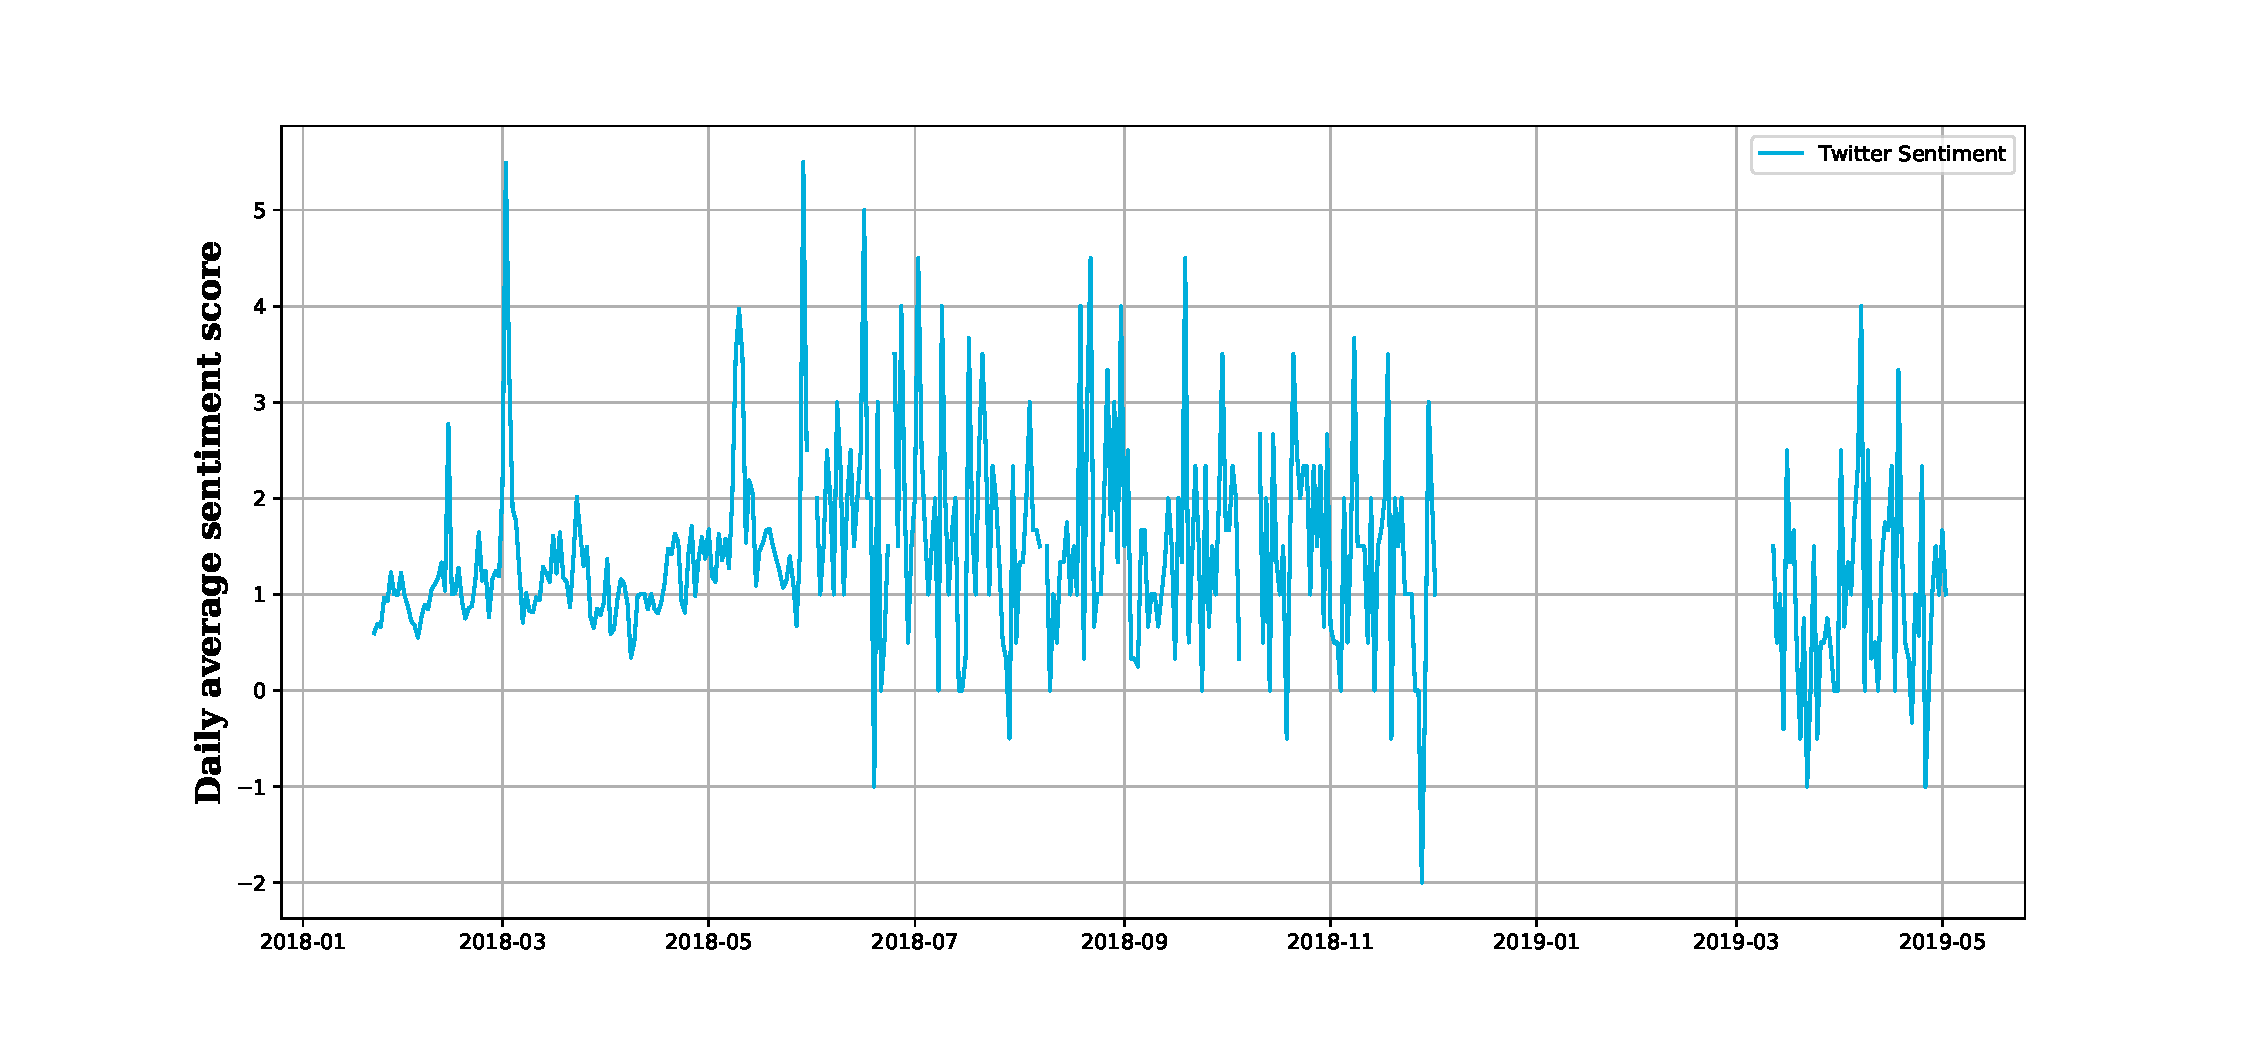
\includegraphics[width=\textwidth]{data/twitter.pdf}
		\caption{ Average Twitter sentiment score regarding the words Ether and Ethereum per day, data source in \cite{deepblueai}. Data for the beginning of 2019 not available.} 
		\label{fig:twitter_plot}
	\end{minipage}
	\hfill
	\begin{minipage}[b]{0.85\textwidth}
		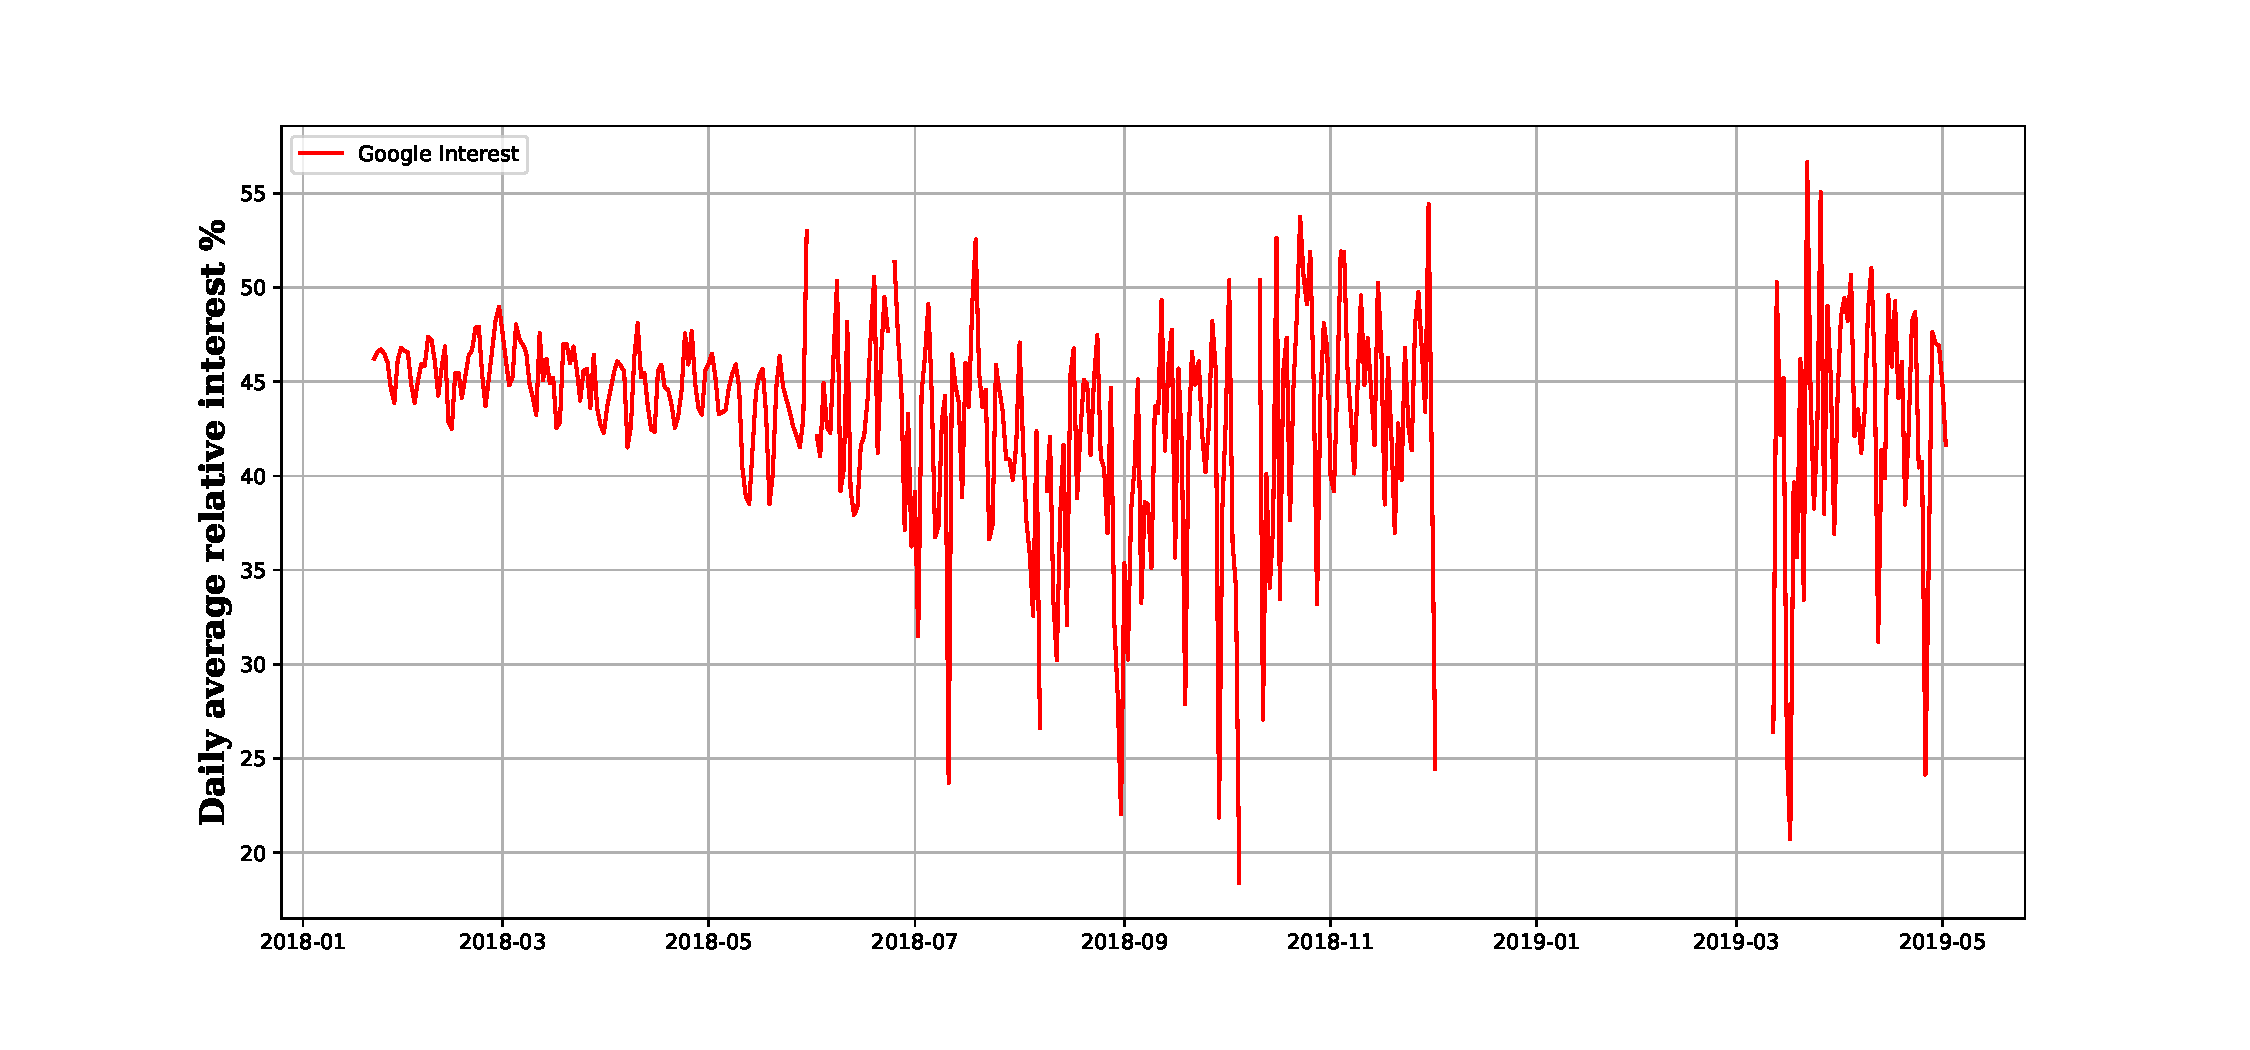
\includegraphics[width=\textwidth]{data/google.pdf}
		\caption{  Average Google trend relative popularity score regarding the words Ether and Ethereum per day, data source in \cite{deepblueai}. Data for the beginning of 2019 not available.}
		\label{fig:google_plot}
	\end{minipage}
\end{figure}


\begin{table}[h!]
	\begin{center}
		\begin{tabular}{||c c c c c||} 
			\hline
			Name & N & $\mu$ & $\sigma$ & Description\\ [0.5ex] 
			\hline\hline
			Price($y_{t}$) & 1379 & 201.86 & 260.35 & USD price. $y_{t}$ $\in \mathbb{R}^{>0}$ \\ 
			\hline
			Transaction($Tr$) & 1379 & 3.20x$10^{5}$ & 3.12x$10^{5}$ & Number of transaction per day. $Tr$ $\in \mathbb{N}^{>0}$  \\ 
			\hline
			Interest($I$) & 360 & 43.17 & 5.64 & Popularity on google search. $I$ $\in [0,100]$  \\
			\hline
			Twitter($Tw$) & 360 & 1.40 & 1.03 & Popularity Score on Twitter.  $Tw$ $\in \mathbb{R}$ \\
			\hline
		\end{tabular}
		\caption{General data statistics.}
		\label{table:general_statistics}
	\end{center}
\end{table}


\subsection{Notation and terminology}

We used the notation introduced in the lectures notes of machine learning course for fall 2019 \cite{ml_jacobs_h}. 

A pair-wise sequence of random variables $X,Y$ realizations $(x_{i},y_{i})_{i=1,...,N}$ that come from the joint probability distribution $P_{X,Y}$ with data value spaces $S_{X},S_{Y}$ can be used in a supervised learning task to estimated a decision function  $D:S_{X} \longrightarrow S_{Y}$ from a set of candidates $\mathcal{D}$ that has the lowest empirical $R^{emp}$ commonly known as \emph{training error}. The loss function $L:S_{X} \times S_{Y} \longrightarrow  \mathbb{R}^{>=0}$ is a measure of the cost of miss predicting a realization of $y_{i}$ with a decision function $D$. One last important concept is the notion of $Risk$ or \emph{test error}, which is defined as the expected loss over the true distribution $P_{X,Y}$.

\begin{equation}
R^{emp}(D)= \frac{1}{N} \sum_{i=1}^{N} L(D(x_{i}),y_{i})
\end{equation}

\begin{equation}
D_{opt}= \operatorname*{arg\,min}_{ D \in \mathcal{D} } R^{emp}(D)
\end{equation}

\begin{equation}
L(D(x),y)=||D(x)-y||^2
\label{eq:2_1}
\end{equation}

Unless stated otherwise, we used the \emph{quadratic loss} defined in Equation \ref{eq:2_1} to calculate the $R^{emp}$ to fit the set of parameters $\Theta$ of a giving \emph{Statistical technique}, such as \emph{Ridge regression} for example. However to compare between already fitted models we used \textbf{Cross-validation} to estimate the \emph{test error}. Selecting the proper metric to make this comparison is of crucial importance, unfortunately and as stated in \cite{gneiting2011making} there is not definitive theoretical background for metric selections, and the most commonly used such as mean absolute percentage error $MAPE$, mean square error $MSE$, mean absolute error $MAE$ favors models that under forecast. We, therefore, decided to follow the standard metric used in the M3 competition \cite{makridakis2000m3}, that is, the symmetric mean percentage error $sMAPE$. As shown in \cite{goshima2015estimating}, the  $sMAPE$ can favor under forecasting models in the case of large points error; nonetheless this was not a concern in the present work. The $sMAPE \in [-200,200]$ 

\begin{equation}
sMAPE=\frac{100}{N} \sum_{i=1}^{N}  \frac{|y_{i}-\hat{y}_{i}|}{(|y_{i}|+|\hat{y}_{i}|)/2}
\label{eq:1_6}
\end{equation}






% ==============================================================================
% START: Introduction
% ==============================================================================